Per problemi di classificazione o di previsione vengono utilizzati diversi modelli di machine learning. In questa capitolo verranno descritti brevemete i metodi che verranno utilizzati.
\section{Modelli utilizzati}
\subsection{Random Forest}
\label{ssec:RF}
Il Random Forest(RF) è un algoritmo di supervised classification che consiste in un insieme di metodi basati sul bagging\cite{Random Forest}; è stata usata l'implementazione di \textit{scikit-learn} combina gli alberi facendo la media della loro previsione probabilistica invece di lasciare che ogni albero voti per una singola classe, e supporta intrinsecamente problemi multi-classe.
\subsection{Support Vector Machine}
\label{ssec:SVM}

\subsection{MultiLayer Perceptron}
\label{ssec:MLP}
\section{Metriche}
\label{metrics}
Esistono diverse metriche per valutare i punteggi dei modelli di machine learning. In questo lavoro sono state utilizzate le seguenti metriche:

\begin{enumerate}
    \item \textbf{accuracy}: frazione delle predizioni corretta fatte dal nostro modello, essa è definita come segue
    \begin{equation*} accuracy = \dfrac {(tp + tn)}{(tp + tn + fp + fn)}\end{equation*} 
    dove $tp$, $fn$, $fp$ e $tn$ sono rispettivamente il numero di veri positivi, falsi negativi, falsi positivi, veri negativi
    
    \item \textbf{precision}: capacità del classificatore di non etichettare come positivo un campione che è negativo, definita come segue
    \begin{equation*} precision = \dfrac {tp}{(tp + fp)}\end{equation*} 
    dove $tp$ rappresenta il numero di veri positivi e $fp$ il numero di falsi positivi
    
    \item \textbf{recall}: capacità di un classificatore di trovare tutti i campioni positivi; definita come
    \begin{equation*} recall = \dfrac {tp}{(tp + fn)}\end{equation*} 
    dove $tp$ rappresenta il numero di veri positivi e $fn$ il numero di falsi negativi
    
    \item \textbf{F1-score}: è la media armonica di precision e recall. Varia tra 0 e 1, dove 0 è il peggior punteggio possibile e 1 il migliore. Spesso si utilizza quando si ha a che fare con problemi multi-classe (non binari). La formula per il punteggio F1 è:
    \begin{equation}
       F_1score = 2 * \frac{(precision * recall)}{(precision + recall)}
    \end{equation}
    possiamo dire di avere un buon classificatore quando abbiamo una alta accuracy e una bassa recall
    \item \textbf{roc-auc}: The AUC rappresenta l'area sotto la curva (Area Under the Curve) ROC (Receiver Operating Characteristic)~\cite{RocAUC}. La curva ROC, il modo più comune per valutare le performance di classificatori binari, è creata tracciando su di un piano cartesiano i veri positivi e i falsi positivi. I valori di roc auc variano tra 0 e 1, dove 1 rappresenta il perfetto accuracy score.
\end{enumerate}

\section{Universal Sentence Encoder}
\label{ssec:use}
Nell'ambito del'Natural Language Processing sono state introdotte diverse tecniche per comprendere il significato di una parola o di una frase con lo scopo di rispondere a delle domande ~\cite{wu2017visual} alla sentiment analysis ~\cite{kaur2017survey} e altro ancora.

Negli ultimi anni, il word embedding si è affermato come uno dei metodi di rappresentazione più popolari~\cite{bengio2003neural,collobert2008unified,turian2010word}.
La sua capacità sta nel fatto di sapere cogliere il contesto di una parola in un documento , la somiglianza semantica e sintattica, la relazione con altre parole, ecc. La tecnica più popolare in questo campo è la {\tt Word2vec}, presentata in ~\cite{mikolov2013efficient,mikolov2013distributed} ma sono state introdotte anche altre tecniche come {\tt SkipGram}, {\tt CBOW}, {\tt Log-Bilinear language}~\cite{mnih2007three} ecc. Essi usano un oggetto simile alla probabilità condizionale $P(w|c)$, che prevede la parola target $w$ in base al suo contesto $c$. Sono stati utilizzati per una varietà di compiti, ad esempio, l'estrazione di testi legati alla finanza~\cite{wang2019user}, question answering~\cite{yang2019online}.

Il successo dei metodi di rete neurale per il calcolo del word embedding ha motivato i metodi per la generazione di embedding semantici di testi più lunghi, come frasi e paragrafi. Sono metodi per fare embed di una frase completa in uno spazio vettoriale n-dimensionale. I sentence embed ereditano alcune proprietà dai word embed~\cite{arora2016simple}.

Quindi si potrebbe usare l'embed delle frasi per diversi scopi:
\begin{enumerate}
    \item calcolare la matrice di similarità delle frasi basandosi sugli embed
    \item tracciare frasi con una tecnica di mappatura comune
    \item predict some value for the sentence, ad esempio, sentimento espresso nella frase.
\end{enumerate}
Una applicazione del sentence embedding può essere vista inn~\cite{iyyer2015deep}, dove gli autori usano sentence embeddings in sentiment analysis e question answering. In questo campo, un'enorme tendenza è la ricerca degli Universal Embeddings: embeddings che sono pre-addestrati su un grande corpus e possono essere inseriti in una varietà di modelli di compiti a valle (sentimental analysis, classification, translation) per migliorare automaticamente le loro prestazioni incorporando alcune rappresentazioni generali di parole/frasi apprese sul più ampio dataset.

{\tt FastText}~\cite{joulin2016fasttext}, definito e sviluppato dagli stessi autori di {\tt Word2vec}, ha innescato l'esposione della ricerca sullo universal word embeddings. Il miglioramento principale di {\tt FastText} sull'originale {\tt Word2vec} è l'inclusione di n-grammi, che permettono di calcolare le rappresentazioni delle parole per le parole che non sono apparse nei dati di formazione (parole \quotes{fuori dal vocabolario}).

In questo senso, Google ha sviluppato un proprio sentence embedder, chiamato {\tt Universal Sentence Encoder}, che è in grado di gestire un gran numero di compiti nell'elaborazione del linguaggio naturale~\cite{USE}. In primo luogo, lo hanno sviluppato in lingua inglese, e in secondo luogo, hanno ampliato tale metodo per la contabilità di più di dieci lingue, tra cui italiano, tedesco, spagnolo, ecc~\cite{yang2019multilingue}, e lo hanno reso disponibile su Tensorflow Hub\footnote{\url{https://bit.ly/36BSS52}}. Questa versione multilingua effettua l'embed del testo da 16 lingue in un unico spazio semantico utilizzando un doppio encoder multitasking addestrato che impara le rappresentazioni legate utilizzando, a sua volta, compiti di bridge basati sulla traduzione. L'Universal Sentence Encoder ha dimostrato di mostrare buone prestazioni con una quantità minima di allenamento supervisionato~\cite{USE}; prende in input un testo di lunghezza variabile, e l'uscita è un vettore di 512 dimensioni. In questo lavoro, è stato usato il multilingual Universal Sentence Encoder per effettuare l'embedding di frasi scritte in linguaggio naturale al fine di addestrare un classificatori in grado di riconoscere i topic a cui appartiene la frase e dei classificatori in grado di riconoscere la sensibilità della frase appartenente al topic.


Universal Sentence Encoder(USE) è un encoder che trasforma del testo scritto in linguaggio naturale in un vettore di 512 elementi, questo encoder può essere usato per task di text classification, semantic similarity, clustering e altri task riguardanti l'ambito dell'analisi del testo scritto in linguaggio naturale.\newline
Nel seguente esempio viene mostrato il funzionamento di USE, egli prende in input un testo scritto in linguaggio naturale, codifica la frase in un array di 512 numeri reali, infine è stata misurata la similarità semantica delle frasi codificate.
\begin{figure}[h]
    \centering
    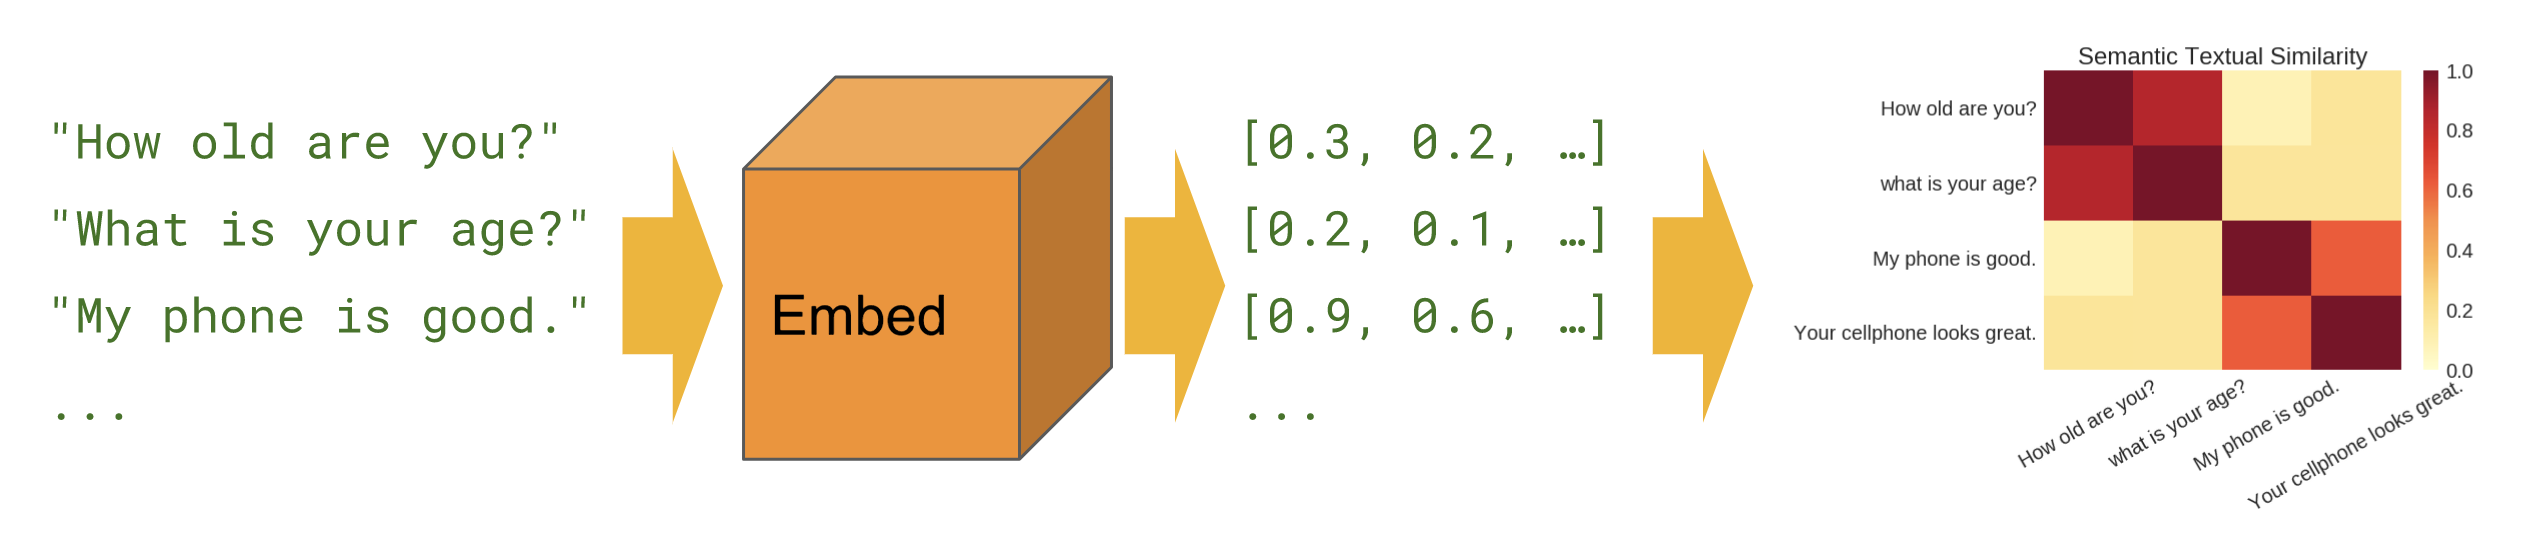
\includegraphics [scale=0.4]{Figure/use.png}
    \caption{Esempio funzionamento USE}
    \label{fig:my_label}
\end{figure}
\FloatBarrier
USE ha vari tipo di encoder, quello utilizzato in questo lavoro è un encoder multilingua che supporta 16 lingue diverse(arabo, cinese-semplificato, cinese-tradizionale, francese, inglese, italiano, giapponese, coreano, olandese, polacco, portoghese, spagnolo, tailandese, turco, russo, tedesco). In questo modo il nostro i modelli che verranno addestrati saranno in grado di riconoscere dati sensibili scritti nelle 16 lingue indicate in precedenza.